\documentclass[a4paper]{article}
\usepackage[affil-it]{authblk}
\usepackage[english]{babel}
\usepackage[backend=bibtex,style=numeric]{biblatex}

\usepackage{geometry}
\geometry{margin=1.5cm, vmargin={0pt,1cm}}
\setlength{\topmargin}{-1cm}
\setlength{\paperheight}{29.7cm}
\setlength{\textheight}{25.3cm}

% useful packages.
\usepackage{amsfonts}
\usepackage{amsmath}
\usepackage{amssymb}
\usepackage{amsthm}     
\usepackage{enumerate} %enumerate environment
\usepackage{graphicx}
\usepackage{multicol}
\usepackage{fancyhdr}
\usepackage{layout}
\usepackage{ctex}      %中文环境
\usepackage{booktabs}  %三线表
\usepackage{verbatim}  %comment environment
\usepackage{float}     %强制表格图片位置
\usepackage{listings}  %insert code in latex
\usepackage{fontspec}  %font support
\usepackage{tikz}
\usepackage{makecell}
\usetikzlibrary{intersections}
\usepackage{arydshln}

\usepackage[colorlinks,linkcolor=blue]{hyperref}
\usepackage{xcolor}
\definecolor{mygreen}{rgb}{0,0.6,0}
\definecolor{lightgrey}{rgb}{0.95,0.95,0.95}
\definecolor{winered}{rgb}{0.5,0,0}
\definecolor{mymauve}{rgb}{0.58,0,0.82}
\lstset{
      backgroundcolor=\color{lightgrey},
      basicstyle             = \ttfamily,
      breakatwhitespace      = false,
      breaklines             = true,
      captionpos             = none,
      commentstyle           = \color{mygreen}\bfseries,
      extendedchars          = false,
      keepspaces             = true,
      keywordstyle           = \color{winered},         % keyword style
      language               = C++,                     % the language of code
      otherkeywords          = {string},
      numberstyle            = \tiny\color{mygray},
      rulecolor              = \color{black},
      showspaces             = false,
      showstringspaces       = false,
      showtabs               = false,
      stepnumber             = 1,
      stringstyle            = \color{mymauve},         % string literal style
      tabsize                = 2,
      title                  = \lstname,
      aboveskip              = 0pt,
      belowskip              = 0pt,
      columns                = flexible
}

% some common command
\newcommand{\dif}{\mathrm{d}}
\newcommand{\avg}[1]{\left\langle #1 \right\rangle}
\newcommand{\norm}[1]{\left\| #1 \right\|}
\newcommand{\difFrac}[2]{\frac{\dif #1}{\dif #2}}
\newcommand{\pdfFrac}[2]{\frac{\partial #1}{\partial #2}}
\newcommand{\OFL}{\mathrm{OFL}}
\newcommand{\UFL}{\mathrm{UFL}}
\newcommand{\fl}{\mathrm{fl}}
\newcommand{\op}{\odot}
\newcommand{\Eabs}{E_{\mathrm{abs}}}
\newcommand{\Erel}{E_{\mathrm{rel}}}
\addbibresource{citation.bib}

\begin{document}
% =================================================
\title{Numerical Analysis chapter 4 theoretical homework}

\author{Zhouyue Qian 3220104074
  \thanks{Electronic address: \texttt{3220104074@edu.zju.cn}}}
\affil{(Information and Computational Science Class 2201), Zhejiang University }


\date{Due time: \today}

\maketitle

%\begin{abstract}
%    The abstract is not necessary for the theoretical homework, 
%    but for the programming project, 
%    you are encouraged to write one.      
%\end{abstract}





% ============================================
\section*{I}
$1.11011101*2^{8}$

\section*{II}
$1.00110011 \cdots *2^{-1} $

\section*{III}
\textbf{Proof:}We donate $x = 1.0 \cdots 0 * \beta^{e}$, then we have 
$$x-x_{L} = 1*\beta^{e-1}*\beta^{-p},\\
x_{R}-x = 1*\beta^{e}*\beta^{-p}.$$

So, we have $\beta (x-x_{L}) = x_{R}-x$.

\section*{IV}
We have $0 \ 01111110\ 00110011001100110011010 = x_{R}>\frac{2}{3}>x_{L} = 0 \ 01111110\ 00110011001100110011001$, the relative error is $3.97*10^{-8}$.

\section*{V}
The older version of $\epsilon_u = \frac{1}{2}*2^{-23} = 2^{-24} $, and the new version of $\epsilon_u = 2^{-23}$. 

\section*{VI}
We need to calculate that $1 - cos(\frac{1}{4})$.
We know that $cos(x) = 1 - \frac{x^2}{2} + \frac{x^4}{4!} - \cdots$, so we have $1 - cos(\frac{1}{4}) = \frac{1}{32}-\frac{1}{6144}+ \cdots$.
During the calculation, we have lost the precision of the last term. We lost $log_2(\frac{1}{32}-\frac{1}{6144})= 5$ digits of precision.

\section*{VII}
\begin{itemize}
    \item $1 - cos(x) = \frac{x^2}{2} - \frac{x^4}{4!} + \cdots$
    \item $1 - cos(x) = 2 sin^{2}(\frac{x}{2}) $
\end{itemize}

\section*{VIII}
As we all know, $\kappa(x) = |\frac{xf'(x)}{f(x)}|$.
\subsection*{a}
$f(x)=(x-1)^{\alpha}, f'(x) = \alpha(x-1)^{\alpha-1}.$ $\kappa(x) = |\frac{\alpha x}{x-1}|$, so when $x \to 1$, $\kappa(x) \to \infty$.
\subsection*{b}
$f(x) = ln(x), f'(x) = \frac{1}{x}$, we have $\kappa(x) = |\frac{1}{lnx}|$, so when $x \to 1$, $\kappa(x) \to \infty$.
\subsection*{c}
We have $\kappa(x)=|x|$, so when $x \to \infty$ , $\kappa(x) \to \infty$.
\subsection*{d}
$f(x)=arccos(x),f'(x) = -\frac{1}{\sqrt{1-x^2} }$, we have $\kappa(x) = |\frac{x}{arccos(x)*\sqrt{1-x^2}}|$, so when $x \to \pm 1$, $\kappa(x) \to \infty$.

\section*{IX}
$f(x)=1 - e^{-x}, x \in [0,1]$
\subsection*{1}
We donate that $a(x) = cond_f(x)=|\frac{xf'(x)}{f(x)}| = |\frac{xe^{-x}}{1-e^{-x}}| = \frac{x}{e^{x}-1}$.$a'(x) = \frac{e^{x}-1-xe^{x}}{(e^{x}-1)^2}$, which means that $a(x)$ is increasing in $[0,1]$.
So, $a(0) = 0, a(1) = \frac{1}{e-1}<1$, which indicates that $cond_f(x)$ is bounded when $x \in [0,1]$. 
\subsection*{2}
From \textbf{Theorem\ 4.78} and question 1, we could know that $f_A(x) = f(x)(1+\delta(x)), |\delta (x)| \leq \varphi (x) \varepsilon_u$, and $cond_A(x) \leq \frac{\varphi (x)}{cond_f(x)}$.
$f_A(x)=fl[fl(1-fl(e^{-fl(x)}))],|\delta_i < \varepsilon_u|$. We know that $e^{-x\delta_1} = 1 - x \delta_1 $.
\begin{align*}
    f_A(x)  &= (1-e^{-x(1+\delta_1)}(1+\delta_2))(1+\delta_3)\\
            &= (1 - e^{-x})(1+\delta_2+\delta_3-x\delta_1 - \frac{\delta_2 - x\delta_1}{1 - e^{-x}})
\end{align*}
We donate $\varphi (x) = 3 + \frac{2}{1 - e^{-x}}$. $\therefore cond_A(x)\leq \frac{\varphi (x)}{cond_f(x)} = \frac{5 - 3e^{-x}}{xe^{-x}}$
\subsection*{3}
Below are figures of $cond_f$ and $cond_A$ 
\begin{figure}[H]
    \centering
    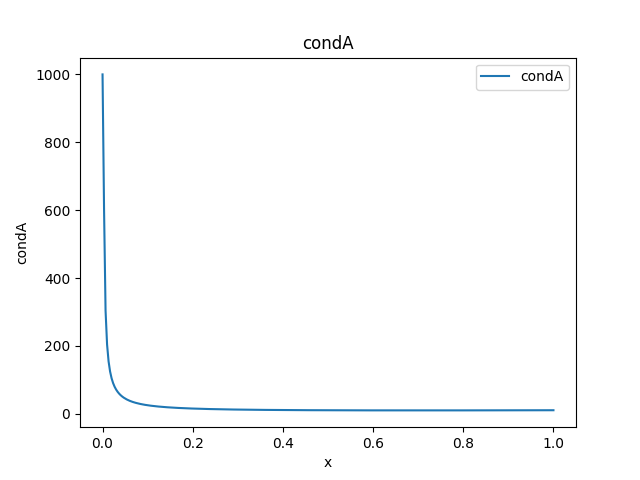
\includegraphics[width=0.8\textwidth]{condA.png}
    \caption{The graph of $cond_A$}
\end{figure}

\begin{figure}[H]
    \centering
    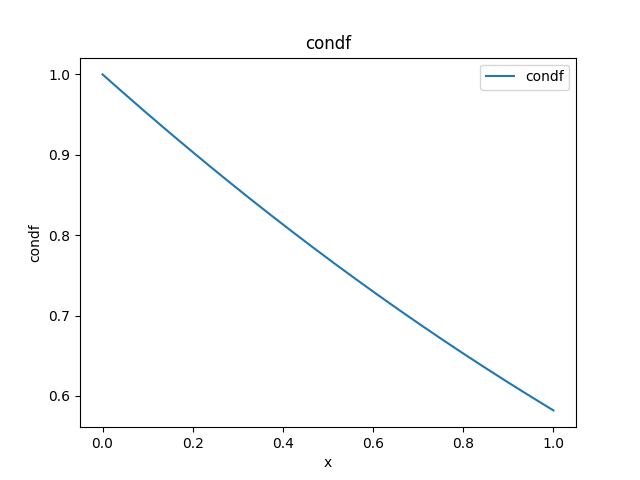
\includegraphics[width=0.8\textwidth]{condf.png}
    \caption{The graph of $cond_f$}
\end{figure}
The result is generated by $Python3$.

\section*{X}
We know that $\| A \|_2 = \sigma_{max} (A)$, also it is easy to know that $\| A^{-1}\|_2 = \sigma_{max} (A^{-1}) = \frac{1}{\sigma_{min} (A)}$.
For the unity matrix, we have $\| I \|_2 = 1$, and $\| I^{-1} \|_2 = 1$, which means that $cond_2(A) = 1$.

\section*{XI}
$q(x) = \sum_{i=0}^{n} a_ix_i, a_n =1 $.
$cond_f(x) = |\frac{1}{r}|\cdot \sum_{i=0}^{n-1}|a_i\frac{\partial r}{\partial a_i}|$,and $\kappa_i(f)=|\frac{1}{r}|\cdot|a_i\frac{\partial r}{\partial a_i}|$.
Now we calculate $\frac{\partial r}{\partial a_i}$, we have $\frac{\partial q}{\partial a_i}+\frac{\partial q}{\partial r} \cdot \frac{\partial r}{\partial a_i} = 0$.
So, we know that $\frac{\partial r}{\partial a_i} = -\frac{r^i}{\sum_{j=1}^{n}ja_jr^{j-1}}$
$\kappa(x)= max |\frac{r^{i-1}a_i}{p'(r)}|$. Now follow the \text{Wilkinson example},$q(r) = \prod_{i=1}^{n}(x-i)$. $\frac{\mathrm{d} }{\mathrm{d} x} \prod_{i=1}^{n}(x-i) = \sum_{j=1}^{n}\prod_{i\ne j}^{n} (x-i)$.
$\kappa_i(x) = |\frac{r^ia_i}{r\sum_{j=1}^{n}\prod_{i\ne j}^{n} (x-i)}|$
$$cond_f(x) = max_{i}|\frac{a_i p^{i-1}}{(p-1)!}|\geq \frac{\sum_{k=1}^{p}kp^{p-2}}{2(p-1)!} = \frac{(p+1)p^{p-1}}{2(p-1)!}$$

\section*{XII}
We have $(2,2,-1,1)$, $a = (1.0)_2*2^{0}, b =  (1.1)_2*2^{0}$. We have $\frac{a }{b}= \frac{2}{3} = (0.1010 \cdots)$.
When we choose the precision of $2p = 4$: $(0.101)_2 = 1.01*2^{-1}$. $fl(\frac{a}{b})= (1.0)_2*2^{-1} = \frac{1}{2}$.
Now, we calculate the relative error: $E_{rel} = \frac{1}{4} = 2^{-2} = \frac{1}{2}*2^{1-2}=\varepsilon_u$, which contradicts
the conclusion of the model of machine arithmetic.

\section*{XIII}
According to \textbf{IEEE754}, we have learnt that there are 24 bits for the mantissa.
Thinking about the root in range of $[128,129]$, it will be represented as $1.xxx\cdots*2^{7}$, the width of the root is $2^{-n}<10^{-6}$,i.e. $n = 20$. 
\begin{itemize}
    \item The spacing between consecutive single-precision FPNs in this range is determined by the exponent:
    \[
    \text{Spacing} = 2^{7 - 23} = 2^{-16} \approx 1.5 \times 10^{-5}.
    \]
    \item This means the smallest representable interval width in this range is approximately \(1.5 \times 10^{-5}\), which is much larger than \(10^{-6}\).
\end{itemize}
So, we cannot compute the root with absolute accuracy $< 10^{-6}$.

\section*{XIV}
For $s(x) = ax^3+bx^2+cx+d,$ we need to know the values of $s(x),s'(x)$ at the point $x_i,x_{i+1}$. 
Note that $s'(x) = 3ax^2 + 2bx + c,a,b,c,d$ can be calculated by 
\begin{equation*}
    \begin{cases}
        ax_{i}^3+bx_{i}^2+cx_{i}+d = f(x_{i}) \\
        ax_{i+1}^3 + bz_{i+1}^2+cx_{i+1}+d = f(x_{i+1}) \\
        3ax_{i}^2 + 2bx_{i} + c = f'(x_i) \\
        3ax_{i+1}^2 + 2bx_{i+1} + c = f'(x_{+1})
    \end{cases}
    \Leftrightarrow
    \left[
    \begin{matrix}
        x_{i}^3 & x_{i}^2 & x_{i} & 1 \\
        x_{i+1}^3 & x_{i+1}^2 & x_{i+1} & 1 \\
        3x_{i}^2 & 2x_i & 1 & 0 \\
        3x_{i+1}^2 & 2x_{i+1} & 1 & 0
    \end{matrix}
    \right] \left[
    \begin{matrix}
        a \\ b \\ c \\ d
    \end{matrix}
    \right]
    =
    \left[
    \begin{matrix}
        f(x_i) \\ f(x_{i+1}) \\ f'(x_i) \\ f'(x_{i+1})
    \end{matrix}
    \right]
\end{equation*}
Denote the cofficients matrix as A, then the maximal condition number is 
$$
\max cond_f(x) = \left\lVert A\right\rVert _2 \left\lVert A^{-1}\right\rVert _2
= \frac{\sigma_{\max}}{\sigma_{\min}}.
$$
When $x_i \to x_{i+1} $, we have find that $\lambda_{min} \to 0$ so the condition number is $\infty$, whcih means in that case that the problem is ill-conditioned.

% ============================================
% ============================================
\section*{ \center{\normalsize {Acknowledgement}} }
\printbibliography


\end{document}